\chapter{Resultados}
\label{cap:4-resultados}

\section{Estudio estadístico}

Esta sección presenta los resultados fruto del estudio estadístico sobre cuáles son los mejores parámetros de los propuestos en el capítulo anterior para optimizar los resultados del algoritmo evolutivo. Se evalúa cada instancia de las mencionadas en la sección~\ref{subsec:instancias} por separado, aportando un conjunto de gráficas de la evolución del fitness para cada conjunto de parámetros evaluado y una tabla con los resultados numéricos de la comparación entre sí de todos los conjuntos, para averiguar si existe una diferencia estadística en los resultados ofrecidos o, si por el contrario, no hay diferencia apreciable entre emplear una configuración u otra.

\subsection{Instancia S\textsubscript{4}: <<anchieta\_tls\_interior\_lane\_always\_green>>}


Con respecto a los resultados del estudio estadístico de la primera instancia, se puede comprobar en la Figura~\ref{fig:estudio:anchieta_tls_interior_lane_always_green} la evolución del fitness para cada una de las cuatro configuraciones que se plantearon para la instancia. 

Las gráficas revelan claramente un incremento del fitness cuando la población es de 50 individuos, independientemente del cruce empleado, pese a que la mejoría no es especialmente abundante. Así pues, para determinar cual configuración es la mejor, hay que referirse a la Tabla~\ref{tab:estudio:anchieta_tls_interior_lane_always_green}. Aquí figuran todas las configuraciones enfrentadas entre sí en parejas.

En dicha tabla se puede apreciar como, al enfrentar a las configuraciones entre sí, la combinación de cruce \texttt{UniformCrossover} y población de tamaño 50 se coloca como la mejor de todas, puesto que produce (observando la mediana) un fitness más elevado al compararla con tres de las configuraciones, revelándose así como el conjunto de parámetros del algoritmo evolutivo que ofrece mejores resultados. En segunda posición queda el conjunto \texttt{OnePointCrossover} y población de tamaño 50, al haber superado solo a dos de las configuraciones. Finalmente, puede apreciarse como no existe ninguna diferencia en emplear una configuración que tenga 10 individuos con cualquier tipo de cruce. Puede consultarse la clasificación de configuraciones en la Tabla~\ref{tab:rankingS4}.

\begin{table}[h]
\centering
\caption{Ranking de las configuraciones de la instancia S\textsubscript{4}}
\label{tab:rankingS4}
\begin{tabular}{lrrr}
\hline
\multicolumn{1}{l}{\textbf{Configuración}} & \textbf{Victorias (V)} & \textbf{Derrotas (D)} & \textbf{V-D} \\ \hline
UniformCrossover / Pob50                   & 3                      & 0                     & 3            \\ \hline
OnePointCrossover / Pob50                  & 2                      & 1                     & 1            \\ \hline
OnePointCrossover / Pob10                  & 0                      & 2                     & -2           \\ \hline
UniformCrossover / Pob10                   & 0                      & 2                     & -2           \\ \hline
\end{tabular}
\end{table}

\begin{figure}[h]
    \centering
    \begin{subfigure}[t]{.49\textwidth}
      \centering
      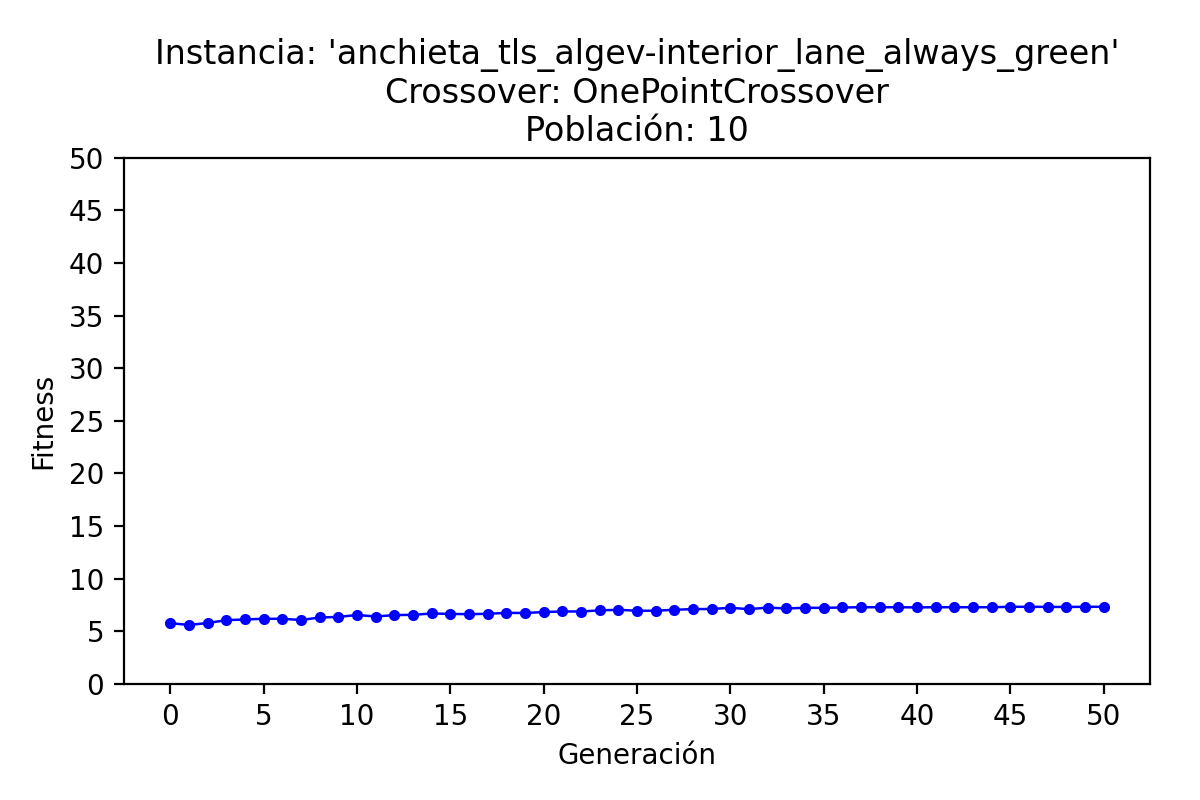
\includegraphics[width=\textwidth]{report/images/estudio/anchieta_tls_algev-interior_lane_always_green-OnePointCrossover-10.png}
    \end{subfigure}
    \hfill
    \begin{subfigure}[t]{.49\textwidth}
      \centering
      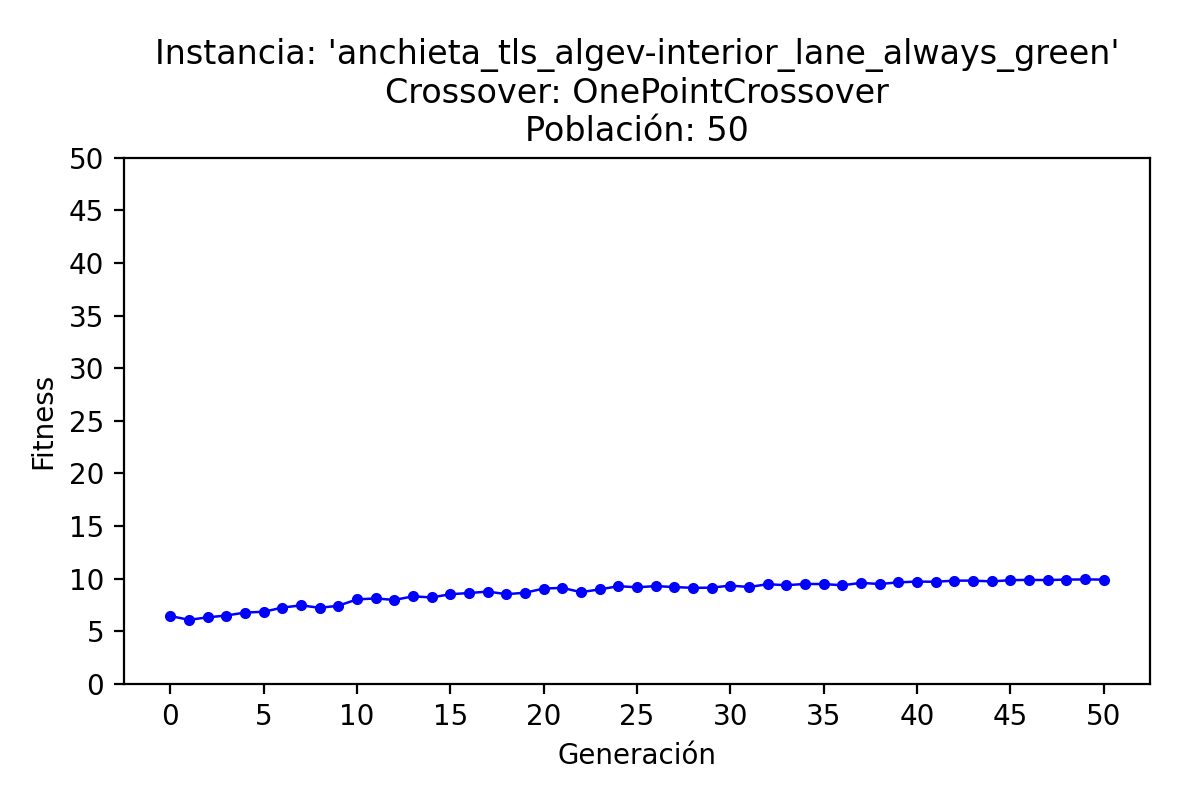
\includegraphics[width=\textwidth]{report/images/estudio/anchieta_tls_algev-interior_lane_always_green-OnePointCrossover-50.png}
    \end{subfigure}
    \vspace{0.7cm}
    \begin{subfigure}[t]{.49\textwidth}
      \centering
      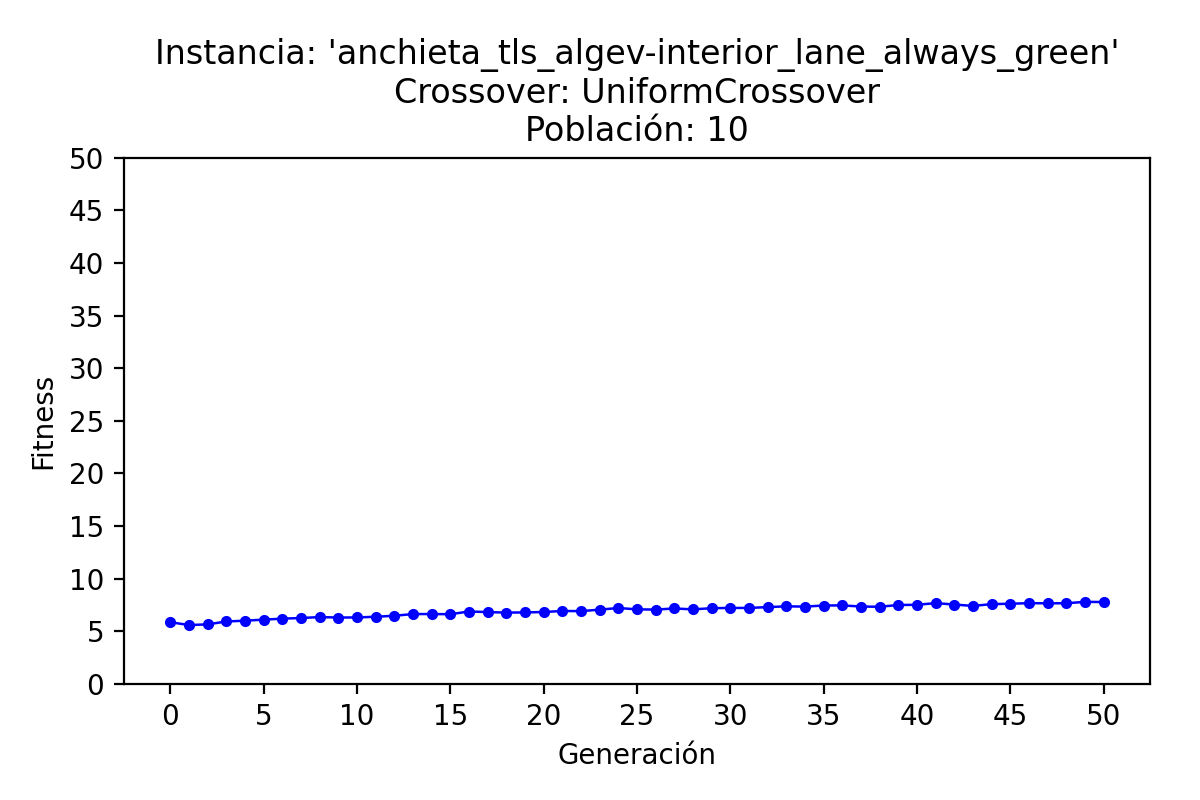
\includegraphics[width=\textwidth]{report/images/estudio/anchieta_tls_algev-interior_lane_always_green-UniformCrossover-10.png}
    \end{subfigure}
    \hfill
    \begin{subfigure}[t]{.49\textwidth}
      \centering
      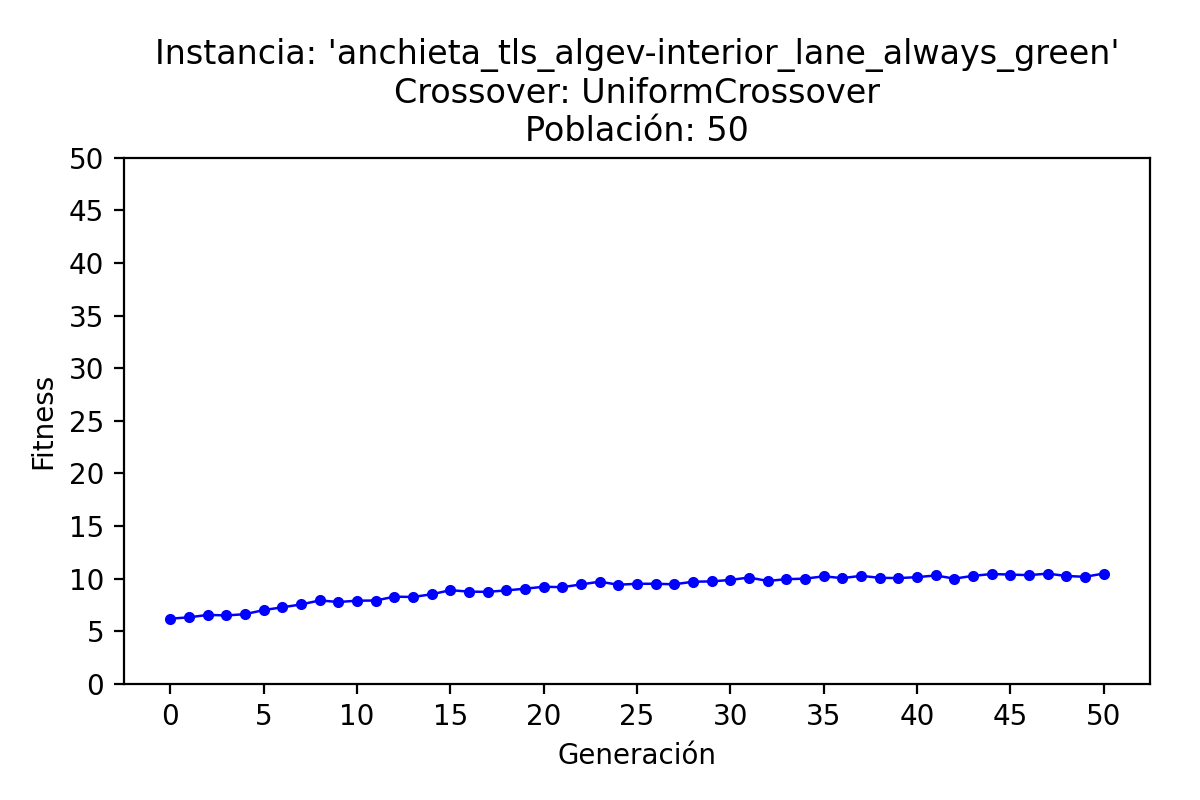
\includegraphics[width=\textwidth]{report/images/estudio/anchieta_tls_algev-interior_lane_always_green-UniformCrossover-50.png}
    \end{subfigure}
    \caption{Evolución del fitness medio entre ejecuciones del mejor candidato de cada generación para la instancia S\textsubscript{4}}
    \label{fig:estudio:anchieta_tls_interior_lane_always_green}
\end{figure}

\subsection{Instancia S\textsubscript{5}: <<anchieta\_tls\_interior\_lane\_changes>>}

Lo cierto es que el estudio de esta instancia arroja resultados similares a los de la instancia anterior. El estudio de la evolución del fitess, que puede apreciarse en la Figura~\ref{fig:estudio:anchieta_tls_interior_lane_changes}, parece resaltar que, al igual que con la instancia anterior, el fitness mejora al usar una población mayor. Sin embargo, esta instancia proporciona de manera general un valor de fitness más alto que la anterior; y en el caso de las comparativas entre cruces, la diferencia en el valor del fitness es más acusada.

Observando los resultados de la evaluación por parejas de las diferentes configuraciones de la Tabla~\ref{tab:estudio:anchieta_tls_interior_lane_changes}, los resultados quedan idénticos a los de la instancia anterior, terminando como ganador el conjunto de parámetros que emplea el cruce \texttt{UniformCrossover} y una población de 50 individuos. En segundo lugar, queda el conjunto \texttt{OnePointCrossover} y población 50 individuos; y de la misma manera, se comprueba que no hay diferencia en emplear uno u otro cruce cuando la población es de 10 individuos. Puede consultarse la clasificación de configuraciones en la Tabla~\ref{tab:rankingS5}.

\begin{table}[h]
\centering
\caption{Ranking de las configuraciones de la instancia S\textsubscript{5}}
\label{tab:rankingS5}
\begin{tabular}{lrrr}
\hline
\multicolumn{1}{l}{\textbf{Configuración}} & \textbf{Victorias (V)} & \textbf{Derrotas (D)} & \textbf{V-D} \\ \hline
UniformCrossover / Pob50                   & 3                      & 0                     & 3            \\ \hline
OnePointCrossover / Pob50                  & 2                      & 1                     & 1            \\ \hline
OnePointCrossover / Pob10                  & 0                      & 2                     & -2           \\ \hline
UniformCrossover / Pob10                   & 0                      & 2                     & -2           \\ \hline
\end{tabular}
\end{table}

\begin{figure}[h]
    \centering
    \begin{subfigure}[t]{.49\textwidth}
      \centering
      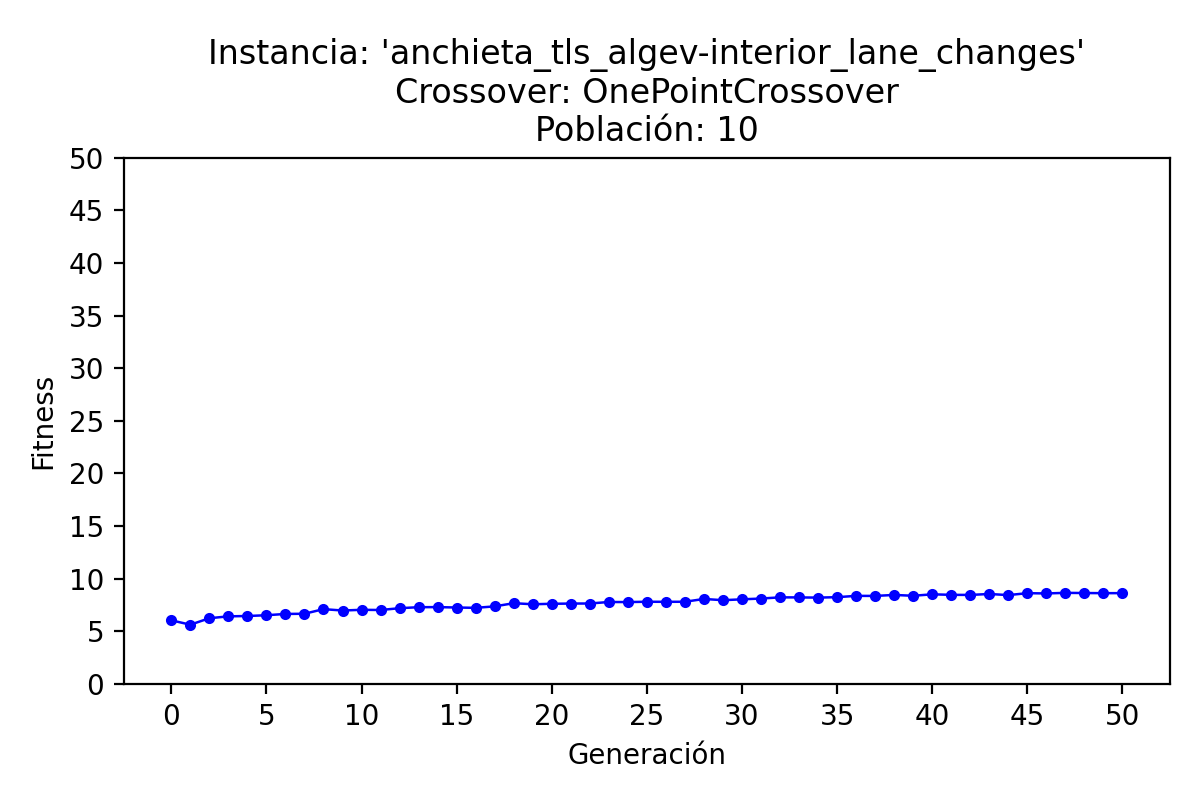
\includegraphics[width=\textwidth]{report/images/estudio/anchieta_tls_algev-interior_lane_changes-OnePointCrossover-10.png}
    \end{subfigure}
    \hfill
    \begin{subfigure}[t]{.49\textwidth}
      \centering
      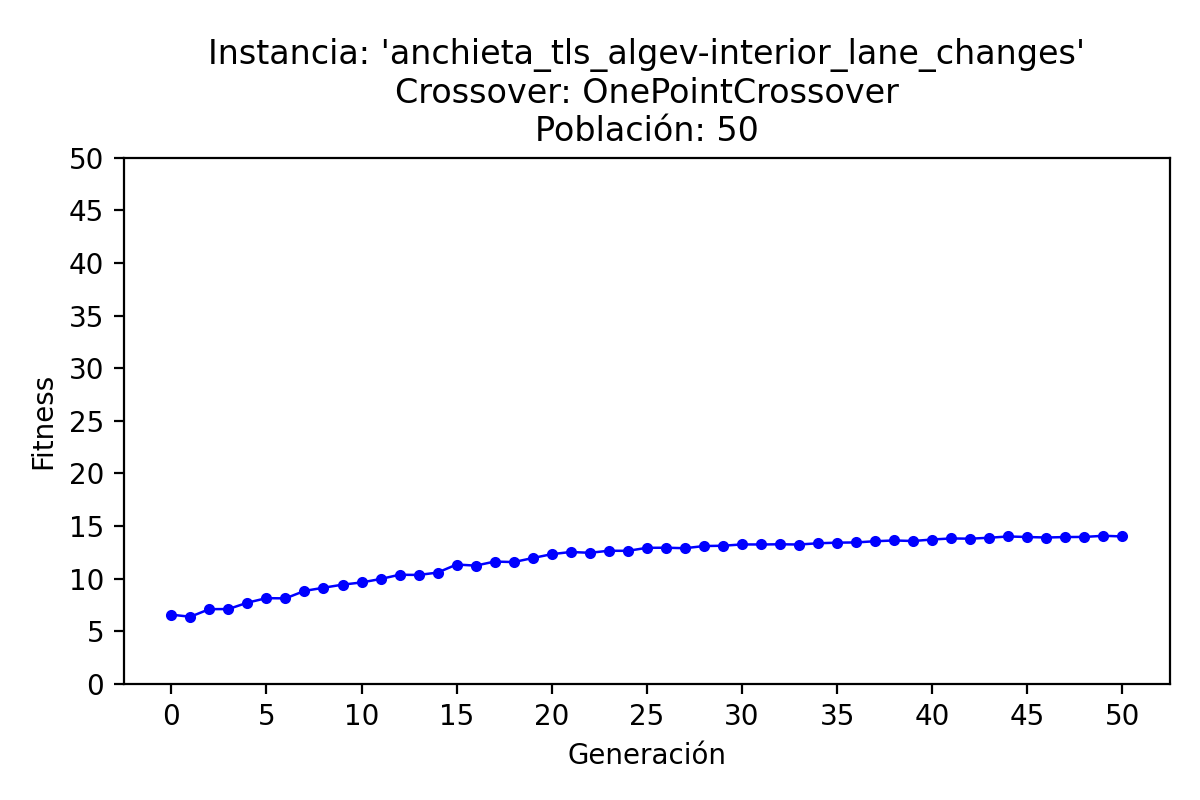
\includegraphics[width=\textwidth]{report/images/estudio/anchieta_tls_algev-interior_lane_changes-OnePointCrossover-50.png}
    \end{subfigure}
    \vspace{0.7cm}
    \begin{subfigure}[t]{.49\textwidth}
      \centering
      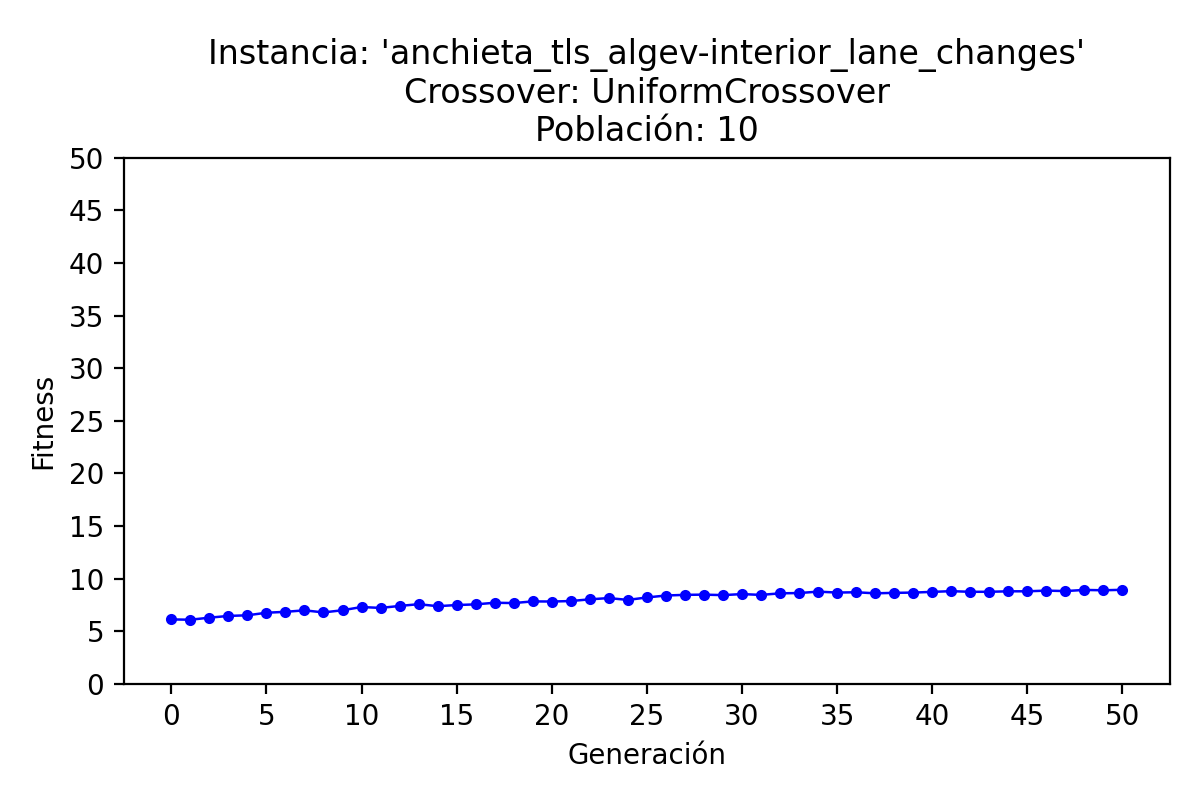
\includegraphics[width=\textwidth]{report/images/estudio/anchieta_tls_algev-interior_lane_changes-UniformCrossover-10.png}
    \end{subfigure}
    \hfill
    \begin{subfigure}[t]{.49\textwidth}
      \centering
      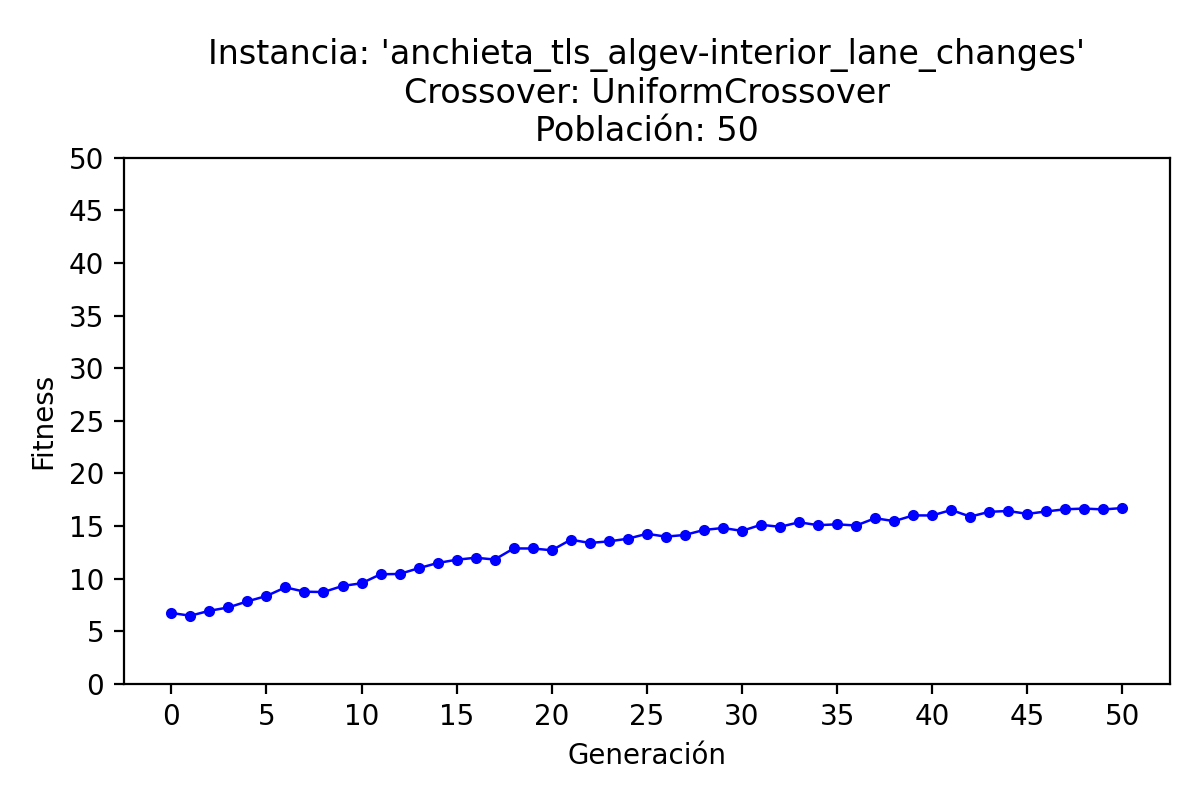
\includegraphics[width=\textwidth]{report/images/estudio/anchieta_tls_algev-interior_lane_changes-UniformCrossover-50.png}
    \end{subfigure}
    \caption{Evolución del fitness medio entre ejecuciones del mejor candidato de cada generación para la instancia S\textsubscript{5}}
    \label{fig:estudio:anchieta_tls_interior_lane_changes}
\end{figure}



\subsection{Instancia S\textsubscript{6}: <<anchieta\_tls\_few\_pedestrians>>}

En comparación con las anteriores, los resultados de la evaluación del fitness de esta instancia (Figura~\ref{fig:estudio:anchieta_tls_special_few_pedestrians}) arrojan resultados mucho mayores; por lo cual se aprecia que la utilización de menos semáforos redunda en un incremento bastante acusado del fitness. Asimismo, y en consonancia con las evaluaciones anteriores, la diferencia en la población se cristaliza una vez más como causante de un incremento en el fitness en el caso de ambos cruces, dando mejores resultados la utilización 50 individuos por generación.

Sin embargo, observando los resultados de la evaluación de los conjuntos de parámetros (Tabla~\ref{tab:estudio:anchieta_tls_special_few_pedestrians}), se puede apreciar como los conjuntos \texttt{OnePointCrossover/Pob50} y \texttt{UniformCrossover/Pob50} llegan a un empate en el cual ambos han ganado (y perdido) la misma cantidad de veces en las evaluaciones con otros conjuntos, además de que no se aprecia diferencia estadística entre uno y otro. Así pues, la conclusión es que realmente no hay diferencia entre emplear cualquiera de los dos, puesto que brindaran resultados extremadamente parecidos. Puede consultarse la clasificación de configuraciones en la Tabla~\ref{tab:rankingS6}.

\begin{table}[h]
\centering
\caption{Ranking de las configuraciones de la instancia S\textsubscript{6}}
\label{tab:rankingS6}
\begin{tabular}{lrrr}
\hline
\multicolumn{1}{l}{\textbf{Configuración}} & \textbf{Victorias (V)} & \textbf{Derrotas (D)} & \textbf{V-D} \\ \hline
UniformCrossover / Pob50                   & 2                      & 1                     & 1            \\ \hline
OnePointCrossover / Pob50                  & 2                      & 1                     & 1            \\ \hline
OnePointCrossover / Pob10                  & 0                      & 2                     & -2           \\ \hline
UniformCrossover / Pob10                   & 0                      & 2                     & -2           \\ \hline
\end{tabular}
\end{table}

\begin{figure}[h]
    \centering
    \begin{subfigure}[t]{.49\textwidth}
      \centering
      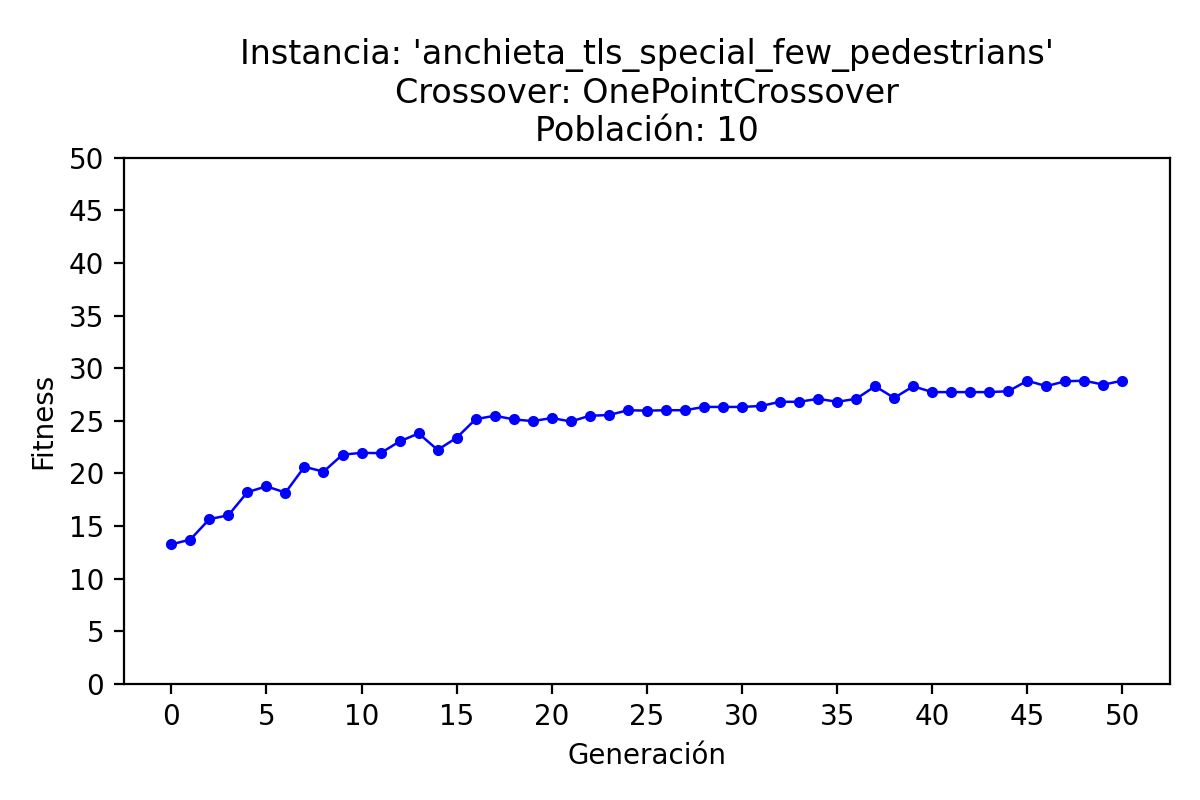
\includegraphics[width=\textwidth]{report/images/estudio/anchieta_tls_special_few_pedestrians-OnePointCrossover-10.png}
    \end{subfigure}
    \hfill
    \begin{subfigure}[t]{.49\textwidth}
      \centering
      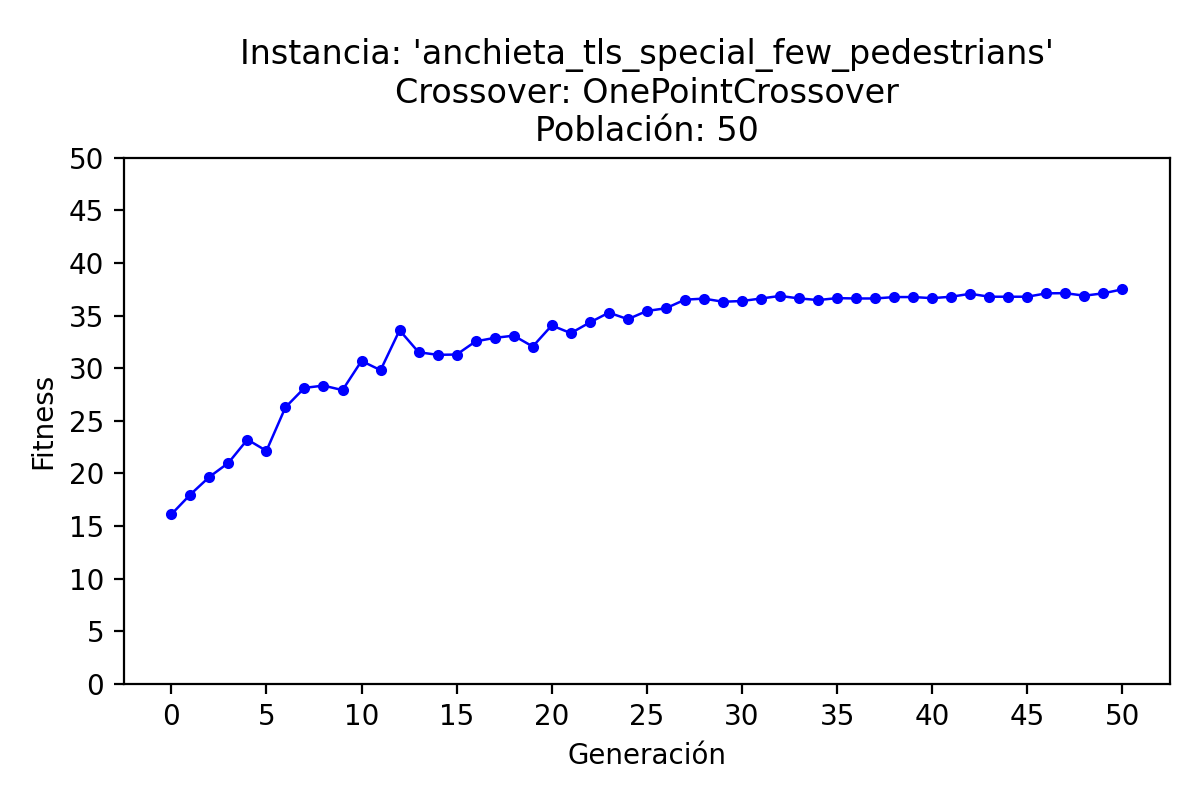
\includegraphics[width=\textwidth]{report/images/estudio/anchieta_tls_special_few_pedestrians-OnePointCrossover-50.png}
    \end{subfigure}
    \vspace{0.7cm}
    \begin{subfigure}[t]{.49\textwidth}
      \centering
      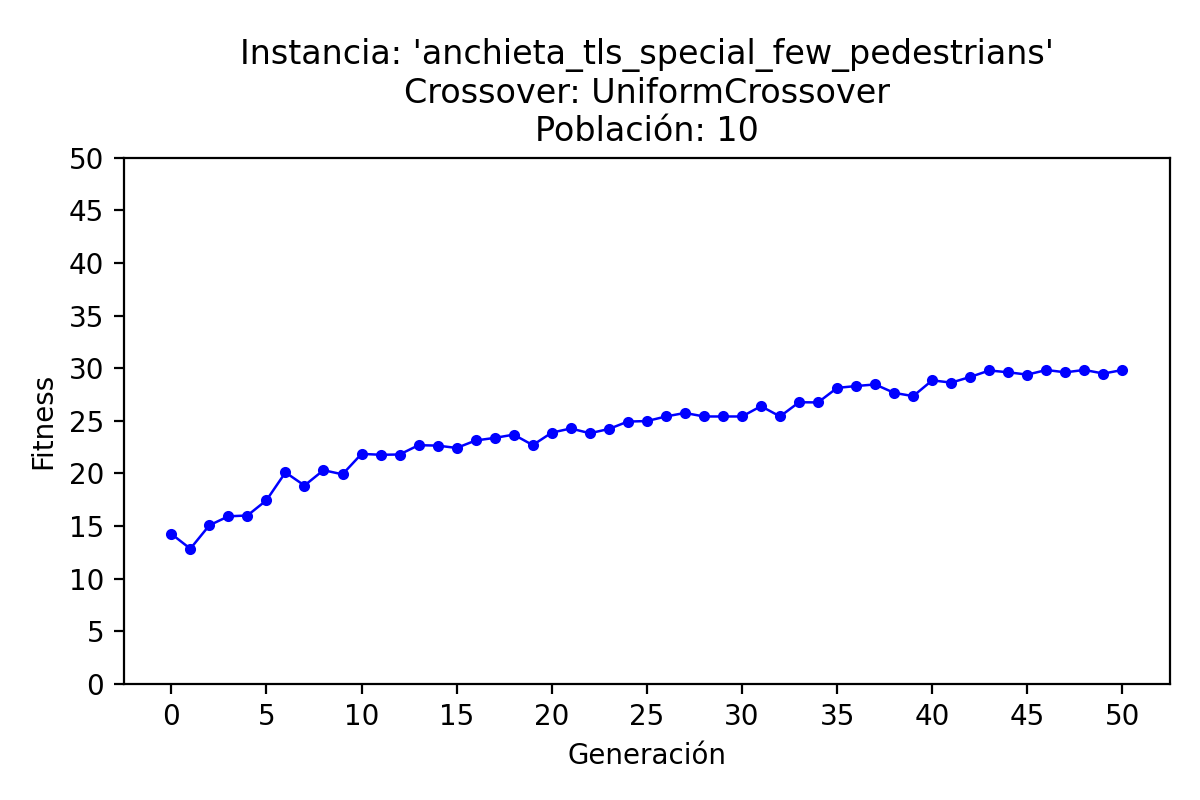
\includegraphics[width=\textwidth]{report/images/estudio/anchieta_tls_special_few_pedestrians-UniformCrossover-10.png}
    \end{subfigure}
    \hfill
    \begin{subfigure}[t]{.49\textwidth}
      \centering
      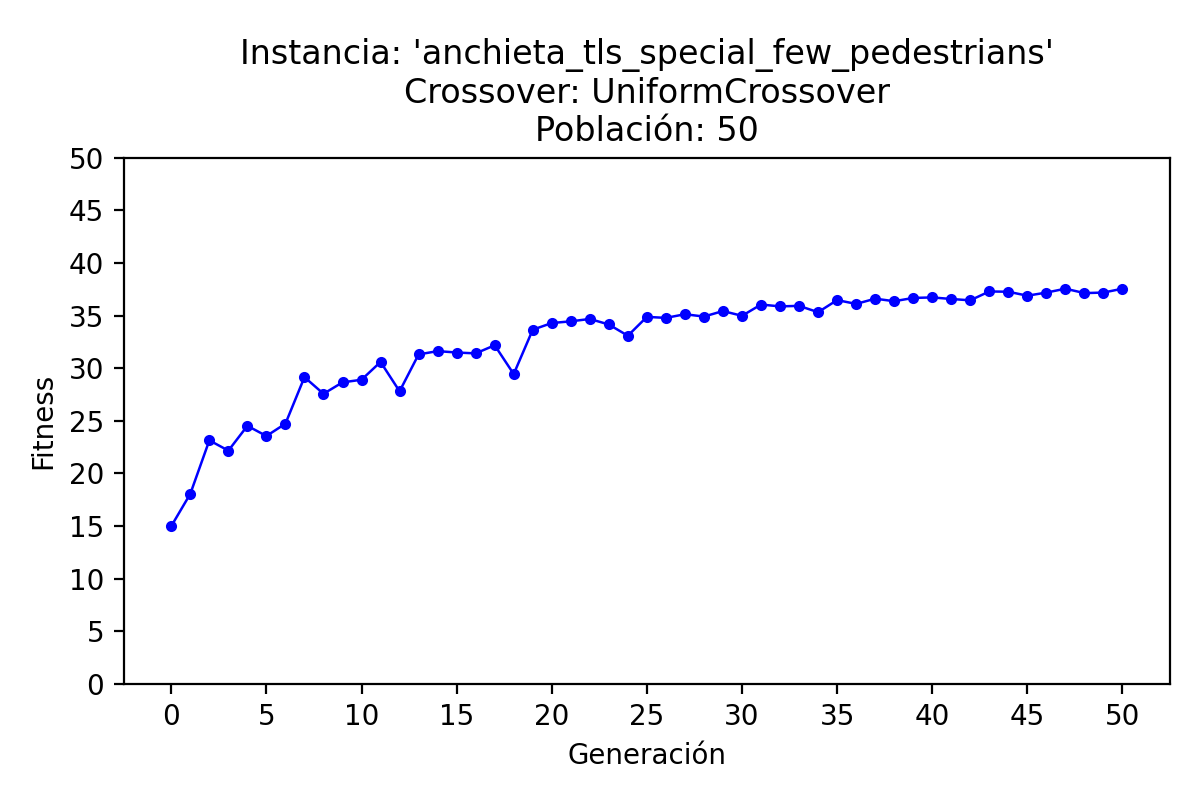
\includegraphics[width=\textwidth]{report/images/estudio/anchieta_tls_special_few_pedestrians-UniformCrossover-50.png}
    \end{subfigure}
    \caption{Evolución del fitness medio entre ejecuciones del mejor candidato de cada generación para la instancia S\textsubscript{6}}
    \label{fig:estudio:anchieta_tls_special_few_pedestrians}
\end{figure}



\subsection{Instancia S\textsubscript{7}: <<anchieta\_tls\_many\_pedestrians>>}

La evaluación del fitness de cada conjunto de parámetros empleado en esta instancia ofrece resultados interesantes si se compara con la anterior, puesto que es fácil apreciar una reducción considerable del fitness en todos los casos, tal y como se puede apreciar en la Figura~\ref{fig:estudio:anchieta_tls_special_many_pedestrians}.  

Observando los resultados de la competición entre sí de cada conjunto (Tabla~\ref{tab:estudio:anchieta_tls_special_many_pedestrians}), se comprueba que los resultados son idénticos a los de la instancia anterior, con un empate entre los conjuntos \texttt{OnePointCrossover/Pob50} y \texttt{UniformCrossover/Pob50}; de modo que no hay diferencia entre emplear uno u otro. Puede consultarse la clasificación de configuraciones en la Tabla~\ref{tab:rankingS7}.

\begin{table}[h]
\centering
\caption{Ranking de las configuraciones de la instancia S\textsubscript{7}}
\label{tab:rankingS7}
\begin{tabular}{lrrr}
\hline
\multicolumn{1}{l}{\textbf{Configuración}} & \textbf{Victorias (V)} & \textbf{Derrotas (D)} & \textbf{V-D} \\ \hline
UniformCrossover / Pob50                   & 2                      & 1                     & 1            \\ \hline
OnePointCrossover / Pob50                  & 2                      & 1                     & 1            \\ \hline
OnePointCrossover / Pob10                  & 0                      & 2                     & -2           \\ \hline
UniformCrossover / Pob10                   & 0                      & 2                     & -2           \\ \hline
\end{tabular}
\end{table}

\begin{figure}[h]
    \centering
    \begin{subfigure}[t]{.49\textwidth}
      \centering
      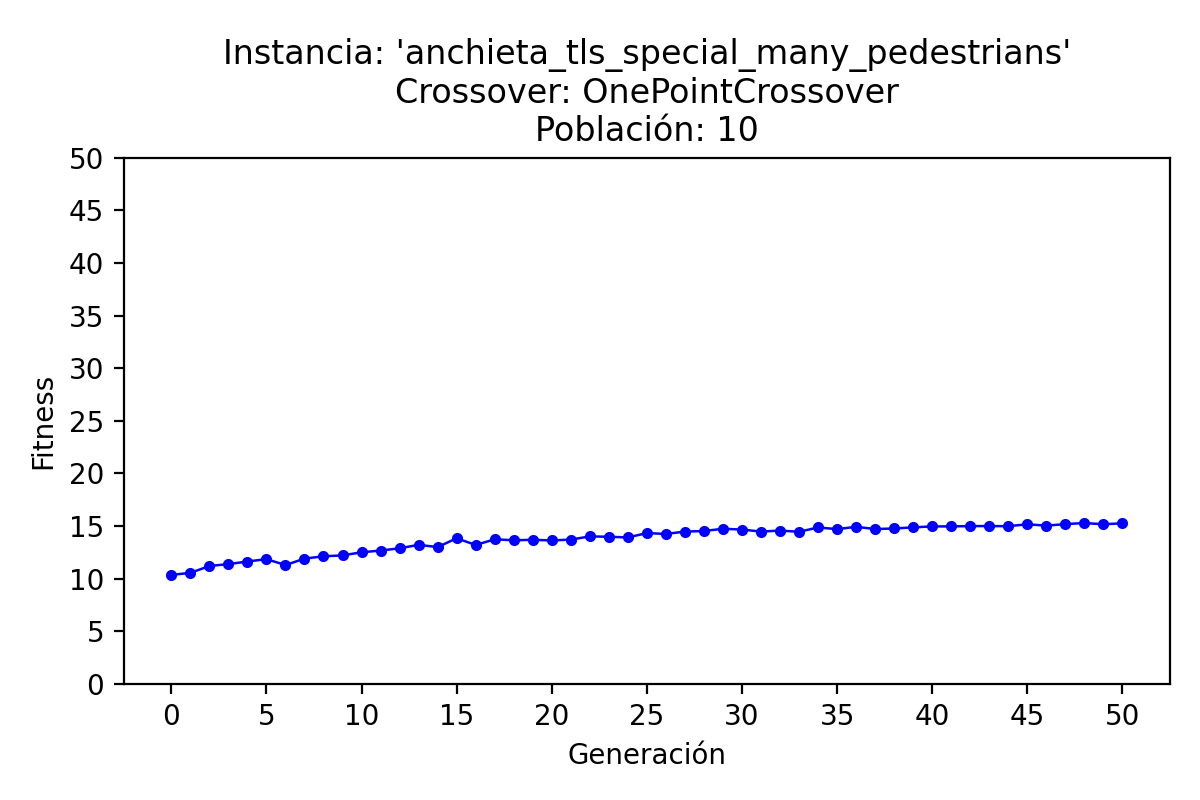
\includegraphics[width=\textwidth]{report/images/estudio/anchieta_tls_special_many_pedestrians-OnePointCrossover-10.png}
    \end{subfigure}
    \hfill
    \begin{subfigure}[t]{.49\textwidth}
      \centering
      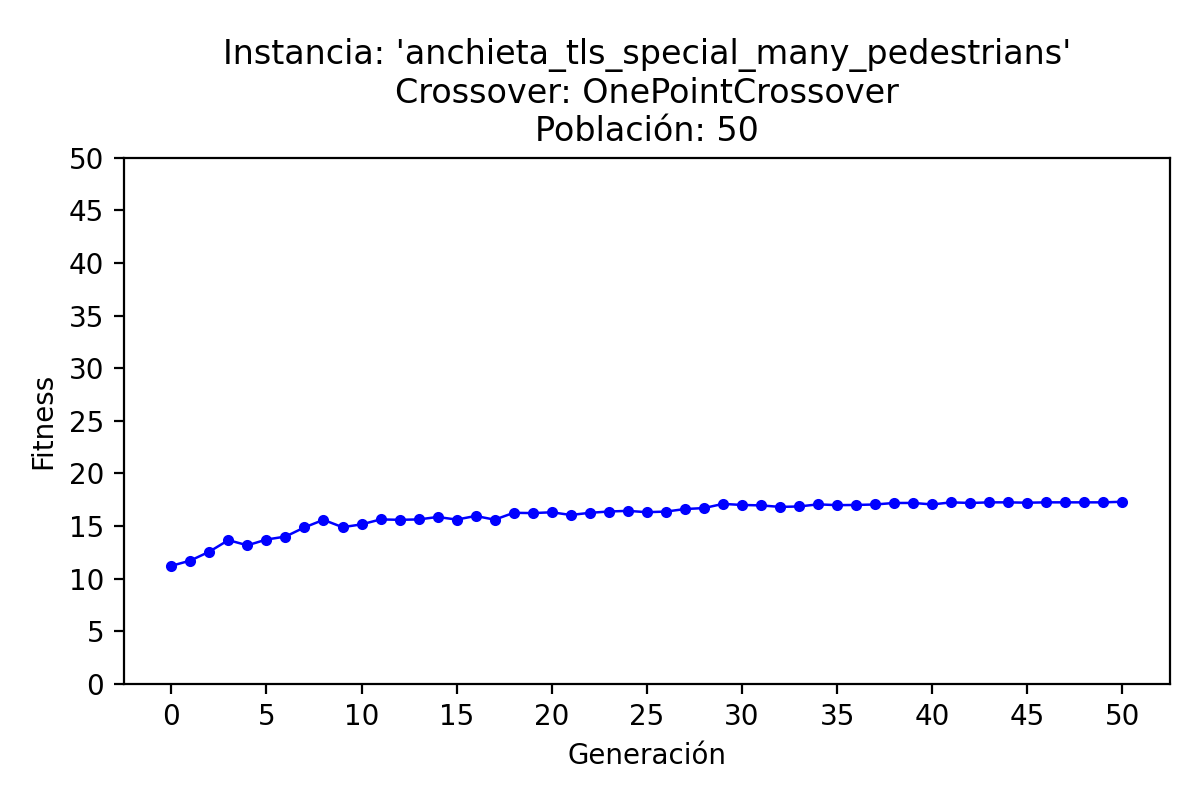
\includegraphics[width=\textwidth]{report/images/estudio/anchieta_tls_special_many_pedestrians-OnePointCrossover-50.png}
    \end{subfigure}
    \vspace{0.7cm}
    \begin{subfigure}[t]{.49\textwidth}
      \centering
      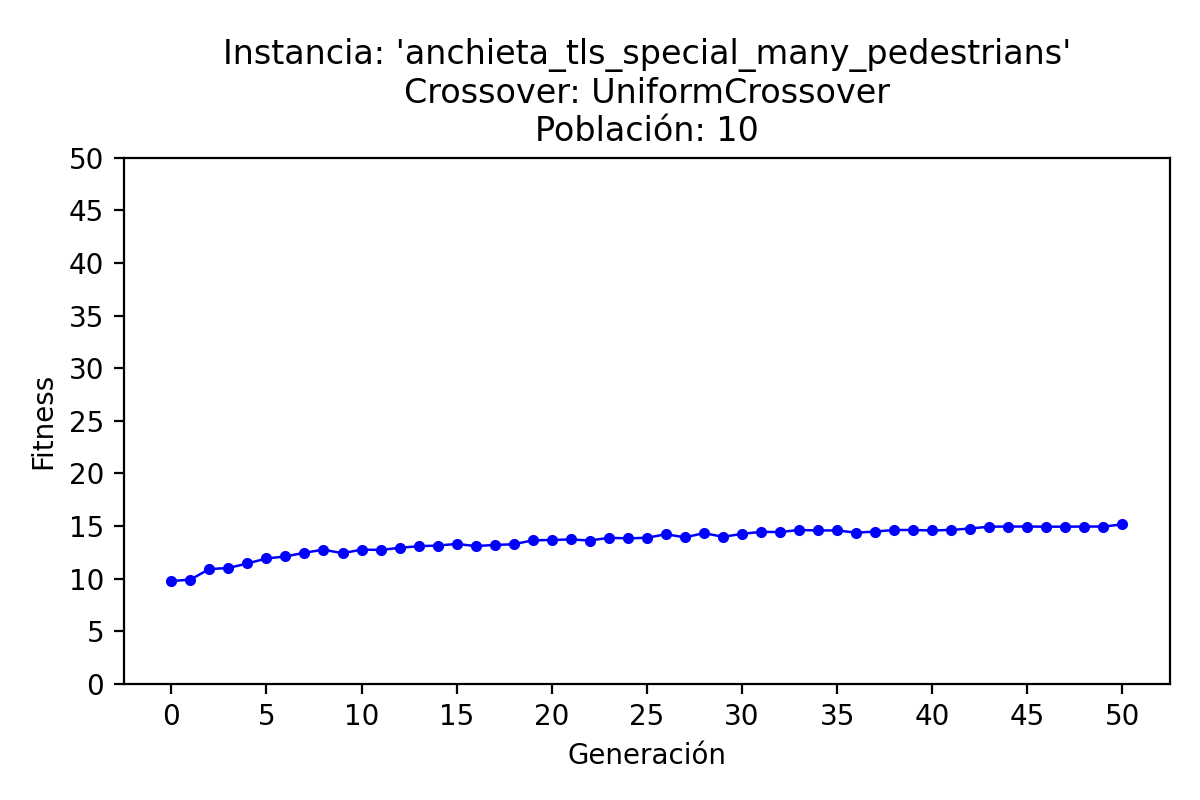
\includegraphics[width=\textwidth]{report/images/estudio/anchieta_tls_special_many_pedestrians-UniformCrossover-10.png}
    \end{subfigure}
    \hfill
    \begin{subfigure}[t]{.49\textwidth}
      \centering
      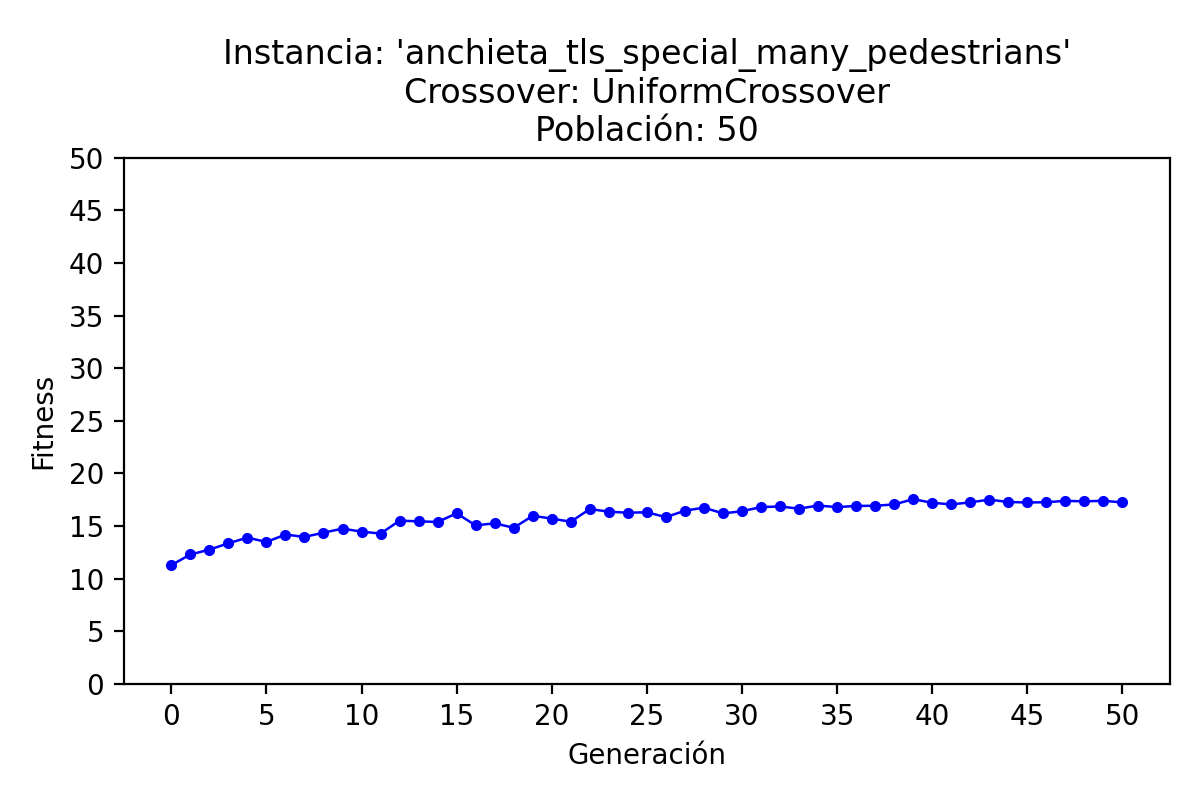
\includegraphics[width=\textwidth]{report/images/estudio/anchieta_tls_special_many_pedestrians-UniformCrossover-50.png}
    \end{subfigure}
    \caption{Evolución del fitness medio entre ejecuciones del mejor candidato de cada generación para la instancia S\textsubscript{7}}
    \label{fig:estudio:anchieta_tls_special_many_pedestrians}
\end{figure}

\begin{sidewaystable}[h]
    \caption{Resultado de la comparación por parejas de la instancia S\textsubscript{4}}
    \label{tab:estudio:anchieta_tls_interior_lane_always_green}
    \resizebox{\textwidth}{!}{\begin{tabular}{lllllll}
    \hline
    \multicolumn{7}{c}{\textbf{anchieta\_tls\_interior\_lane\_always\_green}}                                                                                                                                                                                   \\ \hline
    \multicolumn{1}{c}{\multirow{2}{*}{\textit{Conjuntos de parámetros 1 y 2}}}        & \multicolumn{2}{c}{\textit{Media}}            & \multicolumn{2}{c}{\textit{Mediana}}          & \multicolumn{1}{c}{\multirow{2}{*}{\textit{p-value}}} & \multicolumn{1}{c}{\multirow{2}{*}{\textit{Ganador}}} \\ \cline{2-5}
    \multicolumn{1}{c}{}                                                & \multicolumn{1}{c}{1} & \multicolumn{1}{c}{2} & \multicolumn{1}{c}{1} & \multicolumn{1}{c}{2} & \multicolumn{1}{c}{}                                  & \multicolumn{1}{c}{}                                  \\ \hline
    OnePointCrossover/Pop10 y OnePointCrossover/Pop50                   & 7.364113              & 9.962546              & 7.298901              & 10.05993              & 5.78933e-05                                           & OnePointCrossover/Pop50                               \\ \hline
    OnePointCrossover/Pop10 y UniformCrossover/Pop10                    & 7.364113              & 7.859806              & 7.298901              & 7.632471              & 0.1928009                                             & No hay diferencia estadística                         \\ \hline
    OnePointCrossover/Pop10 y UniformCrossover/Pop50                    & 7.364113              & 11.16813              & 7.298901              & 11.15414              & 0.0001570523                                          & UniformCrossover/Pop50                                \\ \hline
    OnePointCrossover/Pop50 y UniformCrossover/Pop10                    & 9.962546              & 7.859806              & 10.05993              & 7.632471              & 0.0001639967                                          & OnePointCrossover/Pop50                               \\ \hline
    OnePointCrossover/Pop50 y UniformCrossover/Pop50                    & 9.962546              & 11.16813              & 10.05993              & 11.15414              & 0.0101652                                             & UniformCrossover/Pop50                                \\ \hline
    UniformCrossover/Pop10 y UniformCrossover/Pop50                     & 7.859806              & 11.16813              & 7.632471              & 11.15414              & 0.0001570523                                          & UniformCrossover/Pop50                                \\ \hline
    \end{tabular}}
    
    
    
    \bigskip\bigskip\bigskip\bigskip
    \caption{Resultado de la comparación por parejas de la instancia S\textsubscript{5}}
    \label{tab:estudio:anchieta_tls_interior_lane_changes}
    \resizebox{\textwidth}{!}{\begin{tabular}{lllllll}
    \hline
    \multicolumn{7}{c}{\textbf{anchieta\_tls\_interior\_lane\_changes}}                                                                                                                                                                                         \\ \hline
    \multicolumn{1}{c}{\multirow{2}{*}{\textit{Conjuntos de parámetros 1 y 2}}}        & \multicolumn{2}{c}{\textit{Media}}            & \multicolumn{2}{c}{\textit{Mediana}}          & \multicolumn{1}{c}{\multirow{2}{*}{\textit{p-value}}} & \multicolumn{1}{c}{\multirow{2}{*}{\textit{Ganador}}} \\ \cline{2-5}
    \multicolumn{1}{c}{}                                                & \multicolumn{1}{c}{1} & \multicolumn{1}{c}{2} & \multicolumn{1}{c}{1} & \multicolumn{1}{c}{2} & \multicolumn{1}{c}{}                                  & \multicolumn{1}{c}{}                                  \\ \hline
    OnePointCrossover/Pop10 y OnePointCrossover/Pop50                   & 8.654163              & 14.24831              & 8.53437               & 14.10958              & 1.21893e-06                                           & OnePointCrossover/Pop50                               \\ \hline
    OnePointCrossover/Pop10 y UniformCrossover/Pop10                    & 8.654163              & 9.004224              & 8.53437               & 8.693441              & 0.6450571                                             & No hay diferencia estadística                         \\ \hline
    OnePointCrossover/Pop10 y UniformCrossover/Pop50                    & 8.654163              & 17.58131              & 8.53437               & 17.49452              & 1.79459e-09                                           & UniformCrossover/Pop50                                \\ \hline
    OnePointCrossover/Pop50 y UniformCrossover/Pop10                    & 14.24831              & 9.004224              & 14.10958              & 8.693441              & 2.836182e-06                                          & OnePointCrossover/Pop50                               \\ \hline
    OnePointCrossover/Pop50 y UniformCrossover/Pop50                    & 14.24831              & 17.58131              & 14.10958              & 17.49452              & 0.000899443                                           & UniformCrossover/Pop50                                \\ \hline
    UniformCrossover/Pop10 y UniformCrossover/Pop50                     & 9.004224              & 17.58131              & 8.693441              & 17.49452              & 3.310727e-09                                          & UniformCrossover/Pop50                                \\ \hline
    \end{tabular}}
\end{sidewaystable}



\begin{sidewaystable}[h]
    \bigskip\bigskip
    \caption{Resultado de la comparación por parejas de la instancia S\textsubscript{6}}
    \label{tab:estudio:anchieta_tls_special_few_pedestrians}
    \resizebox{\textwidth}{!}{\begin{tabular}{lllllll}
    \hline
    \multicolumn{7}{c}{\textbf{anchieta\_tls\_few\_pedestrians}}                                                                                                                                                                                             \\ \hline
    \multicolumn{1}{c}{\multirow{2}{*}{\textit{Conjuntos de parámetros 1 y 2}}}        & \multicolumn{2}{c}{\textit{Media}}            & \multicolumn{2}{c}{\textit{Mediana}}          & \multicolumn{1}{c}{\multirow{2}{*}{\textit{p-value}}} & \multicolumn{1}{c}{\multirow{2}{*}{\textit{Ganador}}} \\ \cline{2-5}
    \multicolumn{1}{c}{}                                                & \multicolumn{1}{c}{1} & \multicolumn{1}{c}{2} & \multicolumn{1}{c}{1} & \multicolumn{1}{c}{2} & \multicolumn{1}{c}{}                                  & \multicolumn{1}{c}{}                                  \\ \hline
    OnePointCrossover/Pop10 y OnePointCrossover/Pop50                   & 29.45247              & 37.67554              & 27.4298               & 38.05608              & 0.0002177574                                          & OnePointCrossover/Pop50                               \\ \hline
    OnePointCrossover/Pop10 y UniformCrossover/Pop10                    & 29.45247              & 29.88526              & 27.4298               & 28.53967              & 0.8623907                                             & No hay diferencia estadística                         \\ \hline
    OnePointCrossover/Pop10 y UniformCrossover/Pop50                    & 29.45247              & 38.31307              & 27.4298               & 38.35384              & 0.0003900244                                          & UniformCrossover/Pop50                                \\ \hline
    OnePointCrossover/Pop50 y UniformCrossover/Pop10                    & 37.67554              & 29.88526              & 38.05608              & 28.53967              & 0.00180757                                            & OnePointCrossover/Pop50                               \\ \hline
    OnePointCrossover/Pop50 y UniformCrossover/Pop50                    & 37.67554              & 38.31307              & 38.05608              & 38.35384              & 0.4469909                                             & No hay diferencia estadística                         \\ \hline
    UniformCrossover/Pop10 y UniformCrossover/Pop50                     & 29.88526              & 38.31307              & 28.53967              & 38.35384              & 0.001050841                                           & UniformCrossover/Pop50                                \\ \hline
    \end{tabular}}
    
    \bigskip\bigskip\bigskip\bigskip
    \caption{Resultado de la comparación por parejas de la instancia S\textsubscript{7}}
    \label{tab:estudio:anchieta_tls_special_many_pedestrians}
    \resizebox{\textwidth}{!}{\begin{tabular}{lllllll}
    \hline
    \multicolumn{7}{c}{\textbf{anchieta\_tls\_many\_pedestrians}}                                                                                                                                                                                            \\ \hline
    \multicolumn{1}{c}{\multirow{2}{*}{\textit{Conjuntos de parámetros 1 y 2}}}        & \multicolumn{2}{c}{\textit{Media}}            & \multicolumn{2}{c}{\textit{Mediana}}          & \multicolumn{1}{c}{\multirow{2}{*}{\textit{p-value}}} & \multicolumn{1}{c}{\multirow{2}{*}{\textit{Ganador}}} \\ \cline{2-5}
    \multicolumn{1}{c}{}                                                & \multicolumn{1}{c}{1} & \multicolumn{1}{c}{2} & \multicolumn{1}{c}{1} & \multicolumn{1}{c}{2} & \multicolumn{1}{c}{}                                  & \multicolumn{1}{c}{}                                  \\ \hline
    OnePointCrossover/Pop10 y OnePointCrossover/Pop50                   & 15.3666               & 17.38808              & 15.65755              & 17.53609              & 7.402106e-05                                          & OnePointCrossover/Pop50                               \\ \hline
    OnePointCrossover/Pop10 y UniformCrossover/Pop10                    & 15.3666               & 15.26587              & 15.65755              & 15.11698              & 0.86804                                               & No hay diferencia estadística                         \\ \hline
    OnePointCrossover/Pop10 y UniformCrossover/Pop50                    & 15.3666               & 17.72223              & 15.65755              & 17.9043               & 4.202438e-05                                          & UniformCrossover/Pop50                                \\ \hline
    OnePointCrossover/Pop50 y UniformCrossover/Pop10                    & 17.38808              & 15.26587              & 17.53609              & 15.11698              & 0.001255819                                           & OnePointCrossover/Pop50                               \\ \hline
    OnePointCrossover/Pop50 y UniformCrossover/Pop50                    & 17.38808              & 17.72223              & 17.53609              & 17.9043               & 0.390172                                              & No hay diferencia estadística                         \\ \hline
    UniformCrossover/Pop10 y UniformCrossover/Pop50                     & 15.26587              & 17.72223              & 15.11698              & 17.9043               & 0.0005555893                                          & UniformCrossover/Pop50                                \\ \hline
    \end{tabular}}
\end{sidewaystable}


\subsection{Análisis de los resultados}
\label{subsec:analisis-resultados-configuraciones}

Realizada una evaluación de las configuraciones anteriores y observando cuáles de ellas resultaron ganadoras, para la simulación se emplearán las instancias obtenidas del algoritmo evolutivo con los siguientes conjuntos de parámetros:

\begin{itemize}
    \item (S\textsubscript{4}) \textbf{anchieta\_tls\_interior\_lane\_always\_green:} \texttt{UniformCrossover/Pob50}
    \item (S\textsubscript{5}) \textbf{anchieta\_tls\_interior\_lane\_changes:} \texttt{UniformCrossover/Pob50}
    \item (S\textsubscript{6}) \textbf{anchieta\_tls\_few\_pedestrians:} \texttt{UniformCrossover/Pob50}
    \item (S\textsubscript{7}) \textbf{anchieta\_tls\_many\_pedestrians:} \texttt{UniformCrossover/Pob50}
\end{itemize}

Para las dos últimas instancias, dado que no existe diferencia estadística entre emplear \texttt{UniformCrossover/Pob50} y \texttt{OnePointCrossover/Pob50}, se ha optado por la primera por simple comodidad, dado que es la misma configuración empleada para las dos primeras instancias.


\section{Simulación}

Esta sección presenta los indicadores que se han tenido en cuenta para evaluar la simulación de las instancias y los resultados obtenidos a través de SUMO, que serán analizados para determinar, finalmente, si el empleo de semáforos optimizados mejora, empeora o no afecta al tráfico rodado de la rotonda del Padre Anchieta.

\subsection{Indicadores}

Para ello, se ha tomado cada una de las instancias provistas por el algoritmo evolutivo, el cual ha sido ejecutado con la configuración que se establece en las secciones~\ref{subsec:proceso-estudio} y~\ref{subsec:analisis-resultados-configuraciones}. Posteriormente, se han realizado 10 simulaciones distintas por cada una de las instancias. En cada una de esas simulaciones se ha empleado una semilla distinta para introducir aleatoriedad en la simulación por los motivos mencionados en la sección~\ref{subsec:proceso-estudio}; y finalmente, se han calculado la media de los resultados provistos por SUMO.

Dichos resultados se pueden consultar en la Tabla~\ref{tab:estudio:resultados}, y se evalúan conforme a los siguientes indicadores:

\begin{itemize}
    \item \textbf{Indicadores con respecto a los vehículos.} Han sido calculados en función de los vehículos definidos en el archivo de tráfico mencionado en la sección~\ref{sec:vehiculos}, y representan la media de las 10 simulaciones.
    \begin{itemize}
        \item \textit{Cargados.} Cantidad de vehículos que SUMO ha detectado en el archivo de tráfico.
        \item \textit{Insertados.} Cantidad de vehículos que se han iniciado su trayecto en la simulación.
        \item \textit{En ejecución.} Cantidad de vehículos insertados que, al momento de terminarse la simulación, no habían completado su trayecto.
        \item \textit{A la espera.} Cantidad de vehículos que no se han podido insertar en la simulación debido a la congestión del tráfico.
    \end{itemize}
    
    \item \textbf{Indicadores con respecto a la circulación.} Han sido calculados en función de los vehículos \textit{insertados} y \textit{en ejecución}, y representan la media de las 10 simulaciones.
    \begin{itemize}
        \item \textit{Longitud (m).} Longitud media del trayecto escogido por los vehículos.
        \item \textit{Velocidad (m/s).} Velocidad media del trayecto de los vehículos.
        \item \textit{T. espera (s).} Tiempo medio en el cual un vehículo ha estado parado involuntariamente.
        \item \textit{T. perdido (s).} Tiempo medio perdido debido a conducir más lento de lo deseado (incluye el \textit{tiempo de espera}).
        \item \textit{Duración (s).} Duración media del trayecto.
        \item \textit{Retardo (s).} Tiempo medio de espera de los vehículos que no pudieron insertarse debido a la falta de espacio en en en las vías de circulación al terminarse la simulación.
    \end{itemize}
    
    \item \textbf{Fitness.} Fitness del candidato, calculado según la función especificada en la sección~\ref{subsec:funcion}.
\end{itemize}

\begin{sidewaystable}
    \caption{Resultados de la ejecución de la simulación empleando la configuración óptima}
    \label{tab:estudio:resultados}
    \resizebox{\textwidth}{!}{\begin{tabular}{llllllllllllll}
    \hline
    \multicolumn{14}{c}{\textbf{Resultados de la simulación}}                                                                                                                                                                                                                                                                                                                                                                                                     \\ \hline
    \multicolumn{1}{c}{\multirow{2}{*}{\textit{Instancia}}} & \multicolumn{4}{c}{\textit{Vehículos}}                                                                                             &  & \multicolumn{6}{c}{\textit{Estadísticas}}                                                                                                                                                                            &  & \multirow{2}{*}{\textit{Fitness}} \\ \cline{2-5} \cline{7-12}
    \multicolumn{1}{c}{}                                    & \multicolumn{1}{c}{Cargados} & \multicolumn{1}{c}{Insertados} & \multicolumn{1}{c}{En ejecución} & \multicolumn{1}{c}{A la espera} &  & \multicolumn{1}{c}{Longitud (m)} & \multicolumn{1}{c}{Velocidad (m/s)} & \multicolumn{1}{c}{T. perdido (s)} & \multicolumn{1}{c}{T. espera (s)} & \multicolumn{1}{c}{Duración (s)} & \multicolumn{1}{c}{Retardo (s)} &  &                                   \\ \hline
    (S\textsubscript{1}) anchieta\_no\_tls                                       & 14181.8                      & 13057.8                        & 614.6                            & 1124                            &  & 1705.982                         & 22.99                               & 88.34                              & 145.44                            & 44.94                            & 70.55                           &  & 21.71                             \\ \hline
    (S\textsubscript{2}) anchieta\_no\_tls\_few\_pedestrians                     & 14182.8                      & 12904.8                        & 623.4                            & 1278                            &  & 1713.93                          & 23.253                              & 91.304                             & 148.404                           & 50.476                           & 71.458                          &  & 18.85                             \\ \hline
    (S\textsubscript{3}) anchieta\_no\_tls\_many\_pedestrians                    & 14182.7                      & 12878.1                        & 640.1                            & 1304.6                          &  & 1707.695                         & 23.125                              & 94.263                             & 151.237                           & 51.693                           & 80.753                          &  & 17.41                             \\ \hline
    (S\textsubscript{4}) anchieta\_tls\_interior\_lane\_always\_green      & 14184                        & 11954.1                        & 761.8                            & 2229.9                          &  & 1739.027                         & 23.883                              & 145.692                            & 201.943                           & 110.81                           & 85.724                          &  & 7.50                              \\ \hline
    (S\textsubscript{5}) anchieta\_tls\_interior\_lane\_changes            & 14183.6                      & 12397.3                        & 781                              & 1786.3                          &  & 1708.098                         & 23.332                              & 130.275                            & 186.185                           & 91.921                           & 95.318                          &  & 10.59                             \\ \hline
    (S\textsubscript{6}) anchieta\_tls\_few\_pedestrians                & 14181.7                      & 12669.1                        & 678.4                            & 1512.6                          &  & 1726.209                         & 23.32                               & 106.309                            & 163.292                           & 61.791                           & 87.167                          &  & 15.01                             \\ \hline
    (S\textsubscript{7}) anchieta\_tls\_many\_pedestrians               & 14183.1                      & 12699.2                        & 737                              & 1483.9                          &  & 1763.325                         & 23.436                              & 115.69                             & 173.26                            & 71.151                           & 59.275                          &  & 14.09                             \\ \hline
    \end{tabular}}
\end{sidewaystable}


\subsection{Análisis de los resultados}

La instancia que resultados obtiene en todos los indicadores es S\textsubscript{1}, <<anchieta\_no\_tls>>. Es evidente que los excelentes resultados que ofrece esta instancia se deben a la falta de obstáculos al tráfico, puesto que no contiene ni peatones ni semáforos, lo que la coloca a la cabeza con mejor fitness (21.71). El tiempo perdido medio es de 88 segundos, y la duración del trayecto borda los 45 s. Asimismo, la longitud y velocidad media del trayecto se establece en 1,705 km y 23 m/s, evaluadas sobre 13057.8 vehículos insertados de media. La duración media del trayecto y el retardo medio se sitúan, respectivamente, en 45 s y 70.5 s.

La instancia S\textsubscript{2}, <<anchieta\_no\_tls\_few\_pedestrians>>, empeora, como era de esperar, en todos los indicadores; salvo la velocidad media del trayecto. Esto se debe a que menos vehículos que debían circular por la rotonda han podido completar su trayecto o incluso ser insertados. Véase el decremento de los vehículos insertados (-1.1 \%) y el considerable incremento de los vehículos a la espera (+12 \%). Sin embargo, no hay peatones que puedan interferir con el tráfico de la autopista, por lo que las cifras se ven inclinadas a tener más en cuenta a los vehículos que circulan por la TF-5 y menos a los vehículos que circulan a través de la rotonda; de ahí el incremento de la velocidad media (+1 \%) y la longitud media del trayecto (+0.4 \%) con respecto a S\textsubscript{1}. Por otro lado, la congestión sí que se ha notado en el fitness (18.85) y, consecuentemente, en los de tiempo perdido y duración del trayecto, que se han incrementado con respecto a S\textsubscript{1} +3.2 \% y +11 \%, respectivamente.

La instancia S\textsubscript{3}, <<anchieta\_no\_tls\_many\_pedestrians>> ofrece resultados ligeramente peores que los de <<anchieta\_no\_tls\_few\_pedestrians>>, como era de esperar al cuadruplicar la cantidad de peatones. Con respecto a la instancia anterior, menos vehículos fueron insertados (-2 \%), y en cantidad similar empeora el indicadores de vehículos a la espera (+2 \%) y el de vehículos en ejecución (+2.6 \%). Asimismo, se incrementa el tiempo perdido con respecto a S\textsubscript{2} (+3.15 \%) y S\textsubscript{1} (+6.28 \%); y la duración (+2.3 y 13 \%, respectivamente); lo que sitúa al fitness en un valor de 17.41.

Observando los resultados de la simulación de las instancias sin semáforos, es posible concluir que la introducción de peatones hace que la circulación se ralentice de un modo apreciable con apenas 500 peatones (instancia S\textsubscript{2}), causando que 150 vehículos no logren ni siquiera ser insertados en la simulación debido a la congestión del tráfico. Por otro lado, el incremento de los peatones hasta los 2000 (instancia S\textsubscript{3}) no parece causar un gran colapso del tráfico, aunque sí lo empeora.

Pasando a las instancias con semáforos, <<anchieta\_tls\_interior\_lane\_always\_green>> (S\textsubscript{4}) ofrece el peor rendimiento de todas. Si la comparamos con S\textsubscript{3}, los vehículos insertados se reducen en más de 1000, una diferencia del -7.2 \%, un considerable decremento de casi 6 puntos si observamos la relación de S\textsubscript{3} con respecto a S\textsubscript{1} (-1.4 \%), siendo la última que es la que mejores resultados ofrece. El resto de indicadores también empeoran acusadamente en comparación con S\textsubscript{3} (que, recordemos, es la instancia sin semáforos que peor rinde de S\textsubscript{1-3} al ser la que más peatones tiene): se incrementan los vehículos en ejecución (+15.9 \%) y a la espera (+41.5 \%), la longitud media (+1.8 \%), el tiempo perdido medio (+35 \%), la duración media del trayecto (+53.35 \%), y el retardo (+5.8 \%). La velocidad media se incrementa ligeramente, por las mismas razones que las expuestas con respecto a la instancia S\textsubscript{2}. El fitness es, pues, el más bajo de todos: 7.5.

La instancia S\textsubscript{5}, <<anchieta\_tls\_interior\_lane\_changes>>, por el contrario, ofrece resultados sustancialmente mejores que S\textsubscript{4}, pero es la segunda peor instancia si observamos su fitness. En comparación con la instancia anterior, se incrementan los vehículos insertados (+3.5 \%) y en ejecución (+2.5 \%), así como decrementan los vehículos a la espera (19.9 \%), el tiempo perdido medio (-10.3 \%) y la duración media del trayecto (-17.3 \%), pero en absoluto es capaz de competir con la peor de las instancias sin semáforos (S\textsubscript{3}) puesto que su fitness es demasiado bajo en comparación, obteniendo un 10.59.

La instancia S\textsubscript{6}, <<anchieta\_tls\_few\_pedestrians>>, mejora considerablemente en todos los indicadores cuando la comparamos con S\textsubscript{4} y S\textsubscript{5}, pero aún así continúa sin ser una opción viable al compararla con la peor de las instancias sin semáforos (S\textsubscript{3}). Comparada con S\textsubscript{5} incrementa los vehículos insertados (+2.1 \%), mantiene aproximadamente la misma velocidad media, decrementa los vehículos en ejecución (-11.8 \%) y a la espera (-15 \%), el tiempo perdido medio (-18.5 \%), la duración media (-33 \%) y el retardo medio (-8.4 \%), alcanzando un fitness de 15.01. Sin embargo, la imagen es distinta al compararla con S\textsubscript{3}, puesto que queda 2.4 puntos por debajo de esta. Comparando los indicadores entre ambas, S\textsubscript{6} reduce los vehículos insertados (-1.62 \%), incrementa los vehículos a la espera (+13.75 \%), la longitud media (+1.1 \%), el tiempo perdido medio (+11.3 \%), la duración media (+16.3 \%) y el retardo medio (+7.3 \%). La instancia no es capaz de mejorar los indicadores pese a que tiene 4 veces menos peatones que la peor instancia sin semáforos.

Finalmente, la instancia S\textsubscript{7}, <<anchieta\_tls\_many\_pedestrians>> no ofrece resultados mucho más alentadores que S\textsubscript{6}, dado que empeora casi todos sus indicadores, al ser la única diferencia entre ambas el incremento de los peatones. Comparada con S\textsubscript{6}, los vehículos insertados apenas varían, se incrementan los vehículos en ejecución (+8 \%) y decrementan los que están a la espera (-1.9 \%). Es la instancia con mayor longitud media de trayecto (1763 m, +2 \%). Asímismo, se incrementa el tiempo perdido medio (+7.8 \%) y la duración media (+13.2 \%), a la vez que decrementa el retardo (-32 \%). Todo ello nos deja un fitness final de 14.09.

Así pues, evaluadas las cifras anteriores, se pueden alcanzar las siguientes conclusiones:

\begin{enumerate}
    \item De las instancias con semáforos propuestas ninguna consigue mejorar, ni equiparar, el rendimiento de la peor instancia sin semáforos propuesta.
    \item  Comparando instancias idénticas cuya única diferencia es la cantidad de peatones (S\textsubscript{2} y S\textsubscript{3}, así como S\textsubscript{6} y S\textsubscript{7}), es posible apreciar que el incremento de los estos tiene un efecto negativo en el tráfico, como era de prever, puesto que la mayoría de los indicadores se ven afectados negativamente lo que queda reflejado en el valor del fitness. Además, en ambos casos se produce un decremento relativamente similar en el valor del fitness (\textpm0.5).
    \item De las instancias propuestas, las dos que incluyen semáforos en cada entrada y salida de la rotonda (S\textsubscript{4} y S\textsubscript{5}) son las que sin duda peores resultados ofrecen. Se ha podido comprobar que permitir que el carril interior de la rotonda permanezca siempre en verde (en la medida en que los cruces lo permitan) es una configuración que empeora la circulación del tráfico.
\end{enumerate}